% ============================================================================
% Accessibility
% ============================================================================
\DocumentMetadata{
  lang = en-US, 
  pdfstandard = ua-2, 
  tagging = on, 
  tagging-setup = {math/setup=mathml-SE}
}

% ============================================================================
% Document Properties - used on title slide and PDF metadata fields
% ============================================================================
\def\PresTitle{Surface Plates}  % Required - top line of title slide
\def\PresSubtitle{Gauges and Measurement}         % Optional - second line
\def\PresAuthor{Brad Peirson}               % Required - below dividing line
\def\PresInstitute{College of Information Technology and Engineering}       % Optional
\def\PresDate{}                             % Optional
\def\PresKeywords{}                         % Optional - used for hyperref

% Presentation Formatting
% ============================================================================
% ============================================================================
% Class Declaration
% ============================================================================
\documentclass[
        mode = handout,     % Projector = one bullet at a time, Handout = all
        font-size=14pt,     % Only accepts 9, 10, 12, 14, 17, 20
        pdfusetitle         % Pulls \title property from document
    ]
    {ltx-talk}              % ltx-talk class

% ============================================================================
% Custom Colors
% ============================================================================
\usepackage[table]{xcolor}
% Colors from the Baker College Style Guide
%\definecolor{BakerADARed}{RGB}{231, 0, 46}   % #e7002e Official ADA red-doesn't pass WCAG AAA for small text
\definecolor{BakerADARed}{RGB}{181, 0, 36}    % #b50024 Adjusted ADA red-passes WCAG AAA for small text
\definecolor{HoneyYellow}{RGB}{255, 196, 0}   % #ffc400
\definecolor{UpNorthGreen}{RGB}{114, 191, 68} % #72bf44
\definecolor{LakeBlue}{RGB}{134, 183, 227}    % #86b7e3
\definecolor{BakerADI}{RGB}{58, 98, 170}
\definecolor{BakerCIM}{RGB}{217, 35, 47}
\definecolor{BakerBlack}{RGB}{31, 34, 40}     % #1f2228
\definecolor{BakerWhite}{RGB}{255, 255, 255}
\definecolor{BakerRed}{RGB}{239, 0, 48}
\definecolor{Abbey}{RGB}{80, 82, 88}
\definecolor{RollingStone}{RGB}{121, 124, 126}
\definecolor{HitGray}{RGB}{165, 169, 172}
\definecolor{Iron1}{RGB}{201, 206, 209}
\definecolor{Iron}{RGB}{222, 225, 226}
\definecolor{BlackHaze1}{RGB}{237, 240, 240}
\definecolor{BlackHaze}{RGB}{245, 247, 247}

% ============================================================================
% Document Data
% ============================================================================
\title{\PresTitle}
\author{\PresAuthor}
\institute{\PresInstitute}
\date{\PresDate}

%Set up the hyperlink colors
\hypersetup{colorlinks,
    linkcolor=BakerBlack,
    urlcolor=BakerADARed,
    pdfauthor = {\PresAuthor},
    %pdftitle = {\PresentationTopic},   % Title is pulled directly
    pdfsubject = {\PresSubtitle},
    pdfkeywords = {\Keywords},
    pdfcreator = {LaTeX with hyperref package},
    pdfproducer = {LuaLaTeX}
    }

% Map your custom style guide colors to the progress bar aliases
\colorlet{pbcomplete}{BakerADARed}
\colorlet{pbincomplete}{Iron}

\usepackage[most]{tcolorbox}

% ============================================================================
% Footer Format
% ============================================================================
\EditInstance{footer}{std}{
  color         = Abbey,
  separator     = \hfill,
  element-order = {title, institute, framenumber},
  right-hspace  = 3mm,
  left-hspace   = 3mm,
}

% \DeclareInstance{footer}{empty}{
%   element-order = {}
% }

% ============================================================================
% Progress Bar Toggles & Helper Macros
% ============================================================================
\usepackage{xfp}        % Needed for floating point math
\newif\ifprogressbar    % Used to determine whether or not to show the bar
\progressbartrue        % Set the bar to true at the start

% Helper macro to automatically turn off the progress bar inside title/section frames
\newcommand{\makeblindframe}[1]{%
  \progressbarfalse
  #1%
  \progressbartrue
}

% ============================================================================
% Custom Page Formats
% ============================================================================
\let\oldmaketitle\maketitle         % Backup the original maketitle command
\let\oldsection\section             % Backup the original section command
\let\oldsubsection\subsection       % Backup the original subsection command

\makeatletter
\renewcommand{\maketitle}{%
\makeblindframe{%
  \disableglobalbackground
  \slidebackground{PresentationTitleGraphic_2048x1151}%
  \color{white}%
  %\UseInstance{footer}{wallpaper}
  \begin{frame}
    \vspace*{1in}%
      \begin{tcolorbox}[
          enhanced,
          colback=black,       
          colframe=black,      
          opacityfill=0.25,       
          arc=6pt,                
          boxrule=0pt,            
          left=20pt, right=20pt,  
          top=20pt, bottom=20pt,
          width=0.80\textwidth,   
          halign=left             
      ]
          \color{white}%
          % Title (Always visible)
          {\large\bfseries\sffamily \@title}\\[0.5em]%
          
          % Conditional Subtitle
          \ifx\PresSubtitle\empty
          \else
            {\normalsize\sffamily \PresSubtitle}\\[0.5em]%
          \fi
          
          % High-contrast divider line
          {\color{white!80}\rule{0.3\textwidth}{0.8pt}}\\[0.5em]%
          
          % Author (Always visible)
          {\small\sffamily \@author}\\%
          
          % Conditional Institute
          \ifx\PresInstitute\empty
          \else
            {\small\sffamily \PresInstitute}\\%
          \fi
          
          % Conditional Date
          \ifx\PresDate\empty
          \else
            {\small\sffamily \@date}\\%
          \fi
      \end{tcolorbox}%
      \vfill     
  \end{frame}%
  \enableglobalbackground{BG}%
  \color{black}%
  %\UseInstance{footer}{std}
}%
}
\makeatother

% Create a variable container to hold the current section title
\newcommand{\currentsectiontitle}{}

% Redefine \section to take 1 argument (the title)
\renewcommand{\section}[1]{%
\makeblindframe{%
  \renewcommand{\currentsectiontitle}{#1}%
  \disableglobalbackground
  \slidebackground{PresentationSectionBackground_2048x1151}%
  \begin{frame}
    \vfill
    %\vspace*{0.625in}%
    \begin{tcolorbox}[
        enhanced,
        colback=black,       
        colframe=black,      
        opacityfill=0.25,       
        arc=6pt,                
        boxrule=0pt,            
        left=20pt, right=20pt,  
        top=20pt, bottom=20pt,
        width=0.80\textwidth,   
        halign=left             
    ]
        \color{white}%
        {\large\bfseries\sffamily #1}\\[0.5em]%   
    \end{tcolorbox}%
    \vfill 
  \end{frame}%
  \oldsection{#1}%
  \enableglobalbackground{BG}%

  % This will be used for an auto TOC at every section
  % Right now ltx-talk TOC is still in development
  % Once it comes a little further along this can be used
  % \begin{frame}
  %       \frametitle{Section Overview}
  %       \tableofcontents[sections=\thesection]
  %   \end{frame}%
}%
}

% Redefine \subsection to take 1 argument
\renewcommand{\subsection}[1]{%
\makeblindframe{%
  \disableglobalbackground
  \slidebackground{PresentationSectionBackground_2048x1151}%
  \begin{frame}
    \vfill
    %\vspace*{0.25in}% 
    \begin{tcolorbox}[
        enhanced,
        colback=black,       
        colframe=black,      
        opacityfill=0.25,       
        arc=6pt,                
        boxrule=0pt,            
        left=20pt, right=20pt,  
        top=20pt, bottom=20pt,
        width=0.80\textwidth,   
        halign=left             
    ]
        \color{white}%
        {\large\bfseries\sffamily\currentsectiontitle}\\[0.5em]%
        {\normalsize\sffamily #1}%
    \end{tcolorbox}%
    \vfill 
  \end{frame}%
  \oldsubsection{#1}%
  \enableglobalbackground{BG}%
}%
}

%Set the fonts to use NeueHaas Grotesk
\setsansfont{NHAASGROTESKTXPRO-}[
    Path=../NeueHaasGroteskFiles/,
    Scale=1.0,
    Extension = .ttf,
    UprightFont=*55Rg,
    BoldFont=*75Bd,
    ItalicFont=*56It,
    BoldItalicFont=*76BdIt
    ]

% Force the document default family to Sans-Serif
\renewcommand{\familydefault}{\sfdefault}

\usepackage{mathtools} % Load BEFORE unicode math settings
\setmathfont{Fira Math}[Scale=MatchLowercase] 

% 1. Turn global background ON
\newcommand{\enableglobalbackground}[1]{%
  \AddToHook{shipout/background}[mybg]{%
    \put(0, -\paperheight){%
      \includegraphics[width=\paperwidth, height=\paperheight, artifact]{#1}%
    }%
  }%
}

% 2. Turn global background OFF
\newcommand{\disableglobalbackground}{%
  \RemoveFromHook{shipout/background}[mybg]%
}

\newcommand{\slidebackground}[1]{%
  \AddToHookNext{shipout/background}{%
    \put(0, -\paperheight){%
      \includegraphics[width=\paperwidth, height=\paperheight, artifact]{#1}%
    }%
  }%
}

% --- GLOBAL BULLET OVERRIDES ---
\renewcommand{\labelitemi}{\color{BakerBlack}\Large\textbullet}
\renewcommand{\labelitemii}{\color{BakerBlack}\large\textbullet}
\renewcommand{\labelenumi}{\color{BakerBlack}\bfseries\arabic{enumi}.}
\renewcommand{\labelenumii}{\color{BakerBlack}\bfseries\alph{enumii})}

\AddToHook{begindocument/before}{%
  \EditInstance{item}{description}{
    label-format = \normalfont\bfseries\color{BakerADARed}#1
  }%
}

\AddToHook{begindocument/before}{%
  \EditInstance{item}{basic}{
    label-format = \color{BakerADARed}#1
  }%
}

% Global override for ltx-talk slide titles
\EditInstance{frametitle}{header}{
    font = \rule{0pt}{1.5cm}\bfseries\Large,
}

\EditInstance{header}{std}{
    font = \bfseries\huge,
    color = BakerBlack,
}

\AddToHook{env/block/begin}{%
  \colorlet{structure}{BakerADARed}%
}

\pretocmd{\tableofcontents}{\begin{minipage}{\textwidth} \linespread{1.4}}{}{}
\apptocmd{\tableofcontents}{\end{minipage}}{}{}

%Biber not functional in ltx-talk as of 2026-05-29
%Package that allows the creation of bibliographies
\usepackage[
    backend=biber,
    style=authoryear,
    sorting=none,
    %entryhead=false
    ]{biblatex}

%Load the bibliography file
\addbibresource{../../reference.bib}

\defbibheading{bibslide}{References}

\newcolumntype{L}[1]{>{\raggedright\let\newline\\\arraybackslash\hspace{0pt}}m{#1}}
\newcolumntype{C}[1]{>{\centering\let\newline\\\arraybackslash\hspace{0pt}}m{#1}}
\newcolumntype{R}[1]{>{\raggedleft\let\newline\\\arraybackslash\hspace{0pt}}m{#1}}

%All of the graphics are in a seperate folder, this makes it so the folder doesn't have to be repeated every time
\graphicspath{
  {../assets/images}
  {../assets/diagrams}
  {../assets/plots}
}

\makeatletter
% New counter to hold the custom "max frames" for the progress bar
\newcommand{\pb@maxtotal}{1}

% Read the custom total from the .aux file if it exists
\AtBeginDocument{%
  \ifdefined\pb@storedtotal
    \let\pb@maxtotal\pb@storedtotal
  \else
    % Fallback to standard total if our custom hook hasn't run yet
    \edef\pb@maxtotal{\@totalframes}%
  \fi
}

% Custom Appendix command that caps the progress bar and turns it off
\newcommand{\talkappendix}{%
  % 1. Write the CURRENT frame number to the .aux file as the progress total
  \immediate\write\@auxout{\string\gdef\string\pb@storedtotal{\@framenumber}}%
  % 2. Turn off the progress bar for all subsequent appendix slides
  \progressbarfalse
}
\makeatother

% ============================================================================
% Progress Bar Logic 
% ============================================================================
\makeatletter               
\AddToHook{shipout/background}{%
  \ifprogressbar
    % Read ltx-talk's internal frame counter safely
    \edef\currentframe{\@framenumber}%
    \edef\totalframes{\pb@maxtotal}% Use our custom max total instead
    
    % Fallback checks: If the document hasn't fully compiled yet, default to 1
    \ifx\currentframe\empty\def\currentframe{1}\fi
    \ifx\totalframes\empty\def\totalframes{1}\fi
    
    % Draw the progress bar if we have a valid total frame count
    \ifnum\totalframes>1\relax
      % Compute fraction width: (current - 1) / (total - 1)
      \edef\pbfraction{\fpeval{(\currentframe - 1) / (\totalframes - 1)}}%
      
      % Guard rails to prevent the bar from overshooting 100% on a first compile
      \ifdim\pbfraction pt>1pt\def\pbfraction{1}\fi 
      
      \edef\completewidth{\fpeval{\pbfraction * \paperwidth}}%
      \edef\incompletewidth{\fpeval{\paperwidth - \completewidth}}%
      
      % Render full-width progress bar at the top edge
      \put(0cm, -0.1cm){%
        \color{pbcomplete}\rule{\completewidth pt}{2pt}%
        \color{pbincomplete}\rule{\incompletewidth pt}{2pt}%
      }%
    \fi
  \fi
}
\makeatother

% 1. Globally shrink all caption components right as the caption engine fires
\AddToHook{cmd/@makecaption/before}{\footnotesize}

% 2. Declare and assign a blank plug to the kernel's caption label socket
\NewSocketPlug{caption/label}{nolabel}{}
\AssignSocketPlug{caption/label}{nolabel}

\usepackage{adjustbox}

\usepackage{amssymb}
\usepackage{amsmath}
\usepackage{siunitx}

\usepackage{animate}

\usepackage{calc} % Optional, but helpful for layout

\usepackage{multirow}

\usepackage{textcomp}

\usepackage{booktabs}
\usepackage{tabularx}

\usepackage[americanvoltages]{circuitikz}
\usepackage{pgfplots}
\usepackage{pgf-pie}

\usetikzlibrary{
    intersections, 
    fillbetween,
    patterns,
    decorations.pathreplacing,
    decorations.pathmorphing,
    decorations.text,
    decorations.markings,
    arrows.meta,
    arrows,
    shapes,
    shapes.geometric,
    shadows,
    calligraphy,
    backgrounds,
    intersections,
    calc,
    math,
    positioning,
    svg.path,
    shadows,
    shadows.blur,
    spy,
    }

\pgfplotsset{compat=1.18}

\pgfdeclarelayer{ft}
\pgfdeclarelayer{bg}
\pgfsetlayers{bg, main, ft}

% Usage: \hexpic[]{height}{Alt text}{Attribution}{image path}
\newcommand{\hexpic}[5][]{%
  \begin{figure}
    \centering
    \begin{tikzpicture}[
      baseline=(hex.base),      
      every shadow/.style={
        shadow opacity=70
        }
      ]
      \node (hex) [
        draw=white, 
        minimum size=#2, 
        regular polygon, 
        regular polygon sides=6, 
        rotate=90,
        blur shadow
      ] {};
      \begin{scope}
        \clip (hex.corner 1) -- (hex.corner 2) -- (hex.corner 3) -- 
              (hex.corner 4) -- (hex.corner 5) -- (hex.corner 6) -- cycle;
        \node at (hex.center) [#1] {
          \includegraphics[height=#2, alt={#3}]{#5}
        };
      \end{scope}
    \end{tikzpicture}

    \vspace{0.5em}
    {\tiny #4\par}
  \end{figure}  
}

% Usage: \shadowpic[]{width}{Alt text}{Attribution}{image path}
\newcommand{\shadowpic}[5][]{%
  \begin{figure}
    \centering
    \begin{tikzpicture}
      [every shadow/.style={
        shadow opacity=70
        }
      ]
      \node (image) [
        inner sep=0,
        blur shadow
      ] {\includegraphics[width=#2, alt={#3}]{#5}};
    \end{tikzpicture}

    \vspace{0.5em}
    {\tiny #4\par}
  \end{figure}
}

\tikzset{middlearrow/.style={
        decoration={markings, 
        mark= at position 0.5 with {\arrow{#1}},
        },
        postaction={decorate}
    }
}

% Usage: \tikztodo[width]{height}{description/notes}
\newcommand{\tikztodo}[3][0.8\textwidth]{%
  \begin{center}
    \fbox{%
      \parbox[c][#2][c]{#1}{%
        \centering
        \textbf{\textcolor{red}{TODO: TikZ Diagram}}\\[0.5em]
        \small #3%
      }%
    }%
  \end{center}%
}

% Macro: \drawrails{<number_of_1cm_segments>}
\newcommand{\drawrails}[1]{
  % Calculate total depth: 1 cm per segment
  \pgfmathsetmacro{\railheight}{-1 * #1}
  
  % L1 Rail (x = 0)
  \draw[thick] (0, 0) -- (0, \railheight cm);
    
  % L2 Rail (x = 15)
  \draw[thick] (15, 0) -- (15, \railheight cm);
}

\newcommand{\ccwplus}{%
  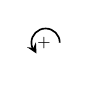
\begin{tikzpicture}[baseline=(char.base)]
    \node(char) at (0,0) {\(\scriptscriptstyle +\)};
    \draw[->, >=stealth, semithick] (0.2,0) arc (0:230:0.18cm);
  \end{tikzpicture}%
}

%====================================================================================
% Timer Ladder Symbol - Could be used for TON, TOF, RTO....
%====================================================================================
\tikzset{
    TON/.pic={

        \draw[
          BakerBlack
        ]
        (0,0)
        -- ++(0,0.375)
        -- ++(3.5,0)
        coordinate[pos=0.5](-TOP)
        -- ++(0,-1.75)
        coordinate[pos=3/14](-OUT)
        coordinate[pos=0.5](-EN1)
        coordinate[pos=0.875](-DN1)
        -- ++(-3.5,0)        
        -- (0,0)
        coordinate(-IN);

        \node[
          text=BakerBlack,
          font=\bfseries,
          anchor=east
        ](pre)
        at ($(-TOP)-(0,1.75em)$)
        {{\small PRE:}};

        \node[
          text=BakerBlack,
          font=\bfseries,
          anchor=east
        ](acc)
        at ($(pre.east)-(0,1em)$)
        {{\small ACC:}};

        \coordinate (-PRE) at (pre.east); % For the preset value
        \coordinate (-ACC) at (acc.east);

        \draw[
            BakerBlack
        ]
        (-EN1)
        -- ++(0.5,0)
        coordinate(-EN2)
        node[
            text=BakerBlack,
            anchor=west
        ]
        {{\small EN}};

        \draw[
            BakerBlack
        ]
        (-DN1)
        -- ++(0.5,0)
        coordinate(-DN2)
        node[
            text=BakerBlack,
            anchor=west
        ]
        {{\small DN}};

    }
}

%====================================================================================
% Oval ladder symbol, good for ONS, RES, etc.
%====================================================================================
\tikzset{
    ONS/.pic={

        \draw[
          BakerBlack
        ]
        (0,0)
        coordinate(-IN)
        -- ++(0.75,0)
        node[
          draw=BakerBlack, 
          text=BakerBlack, 
          font=\small, 
          minimum width=1.5cm, 
          minimum height=0.75cm, 
          anchor=west, 
          rounded corners=0.25cm
          ](ons){};
        
        \draw[BakerBlack] (ons.east) -- ++(0.75,0) coordinate(-OUT);

        \coordinate(-INS) at (ons.center);
        \coordinate(-VAR) at (ons.north); 
    }
}

%====================================================================================
% Source A, Source B, Dest box
%====================================================================================
\tikzset{
    SrcDest/.pic={
      
        \draw[
          BakerBlack
        ]
        (0,0)
        coordinate(-IN)
        -- ++(0,0.375)
        -- ++(5,0)
        coordinate[pos=0.5](-TOP)
        -- ++(0,-3.25)
        coordinate[pos=3/26](-OUT)
        -- ++(-5,0)
        -- (0,0)
        coordinate(l1);

        \node[
          text=BakerBlack,
          font=\bfseries,
          anchor=west
        ](srcA)
        at (l1)
        {{\small Src A:}};

        \node[
          text=BakerBlack,
          font=\bfseries,
          anchor=west
        ](srcB)
        at ($(l1)-(0,2em)$)
        {{\small Src B:}};

        \node[
          text=BakerBlack,
          font=\bfseries,
          anchor=west
        ](dest)
        at ($(srcB.west)-(0,2em)$)
        {{\small Dest:}};

        \coordinate(-SRCA) at (srcA.east);
        \coordinate(-AVAL) at ($(srcA.east)-(0,1em)$);
        \coordinate(-SRCB) at (srcB.east);
        \coordinate(-BVAL) at ($(srcB.east)-(0,1em)$);
        \coordinate(-DEST) at ($(-BVAL)-(0,1em)$);
        \coordinate(-DVAL) at ($(-DEST)-(0,1em)$);
    }
}

%====================================================================================
% Source A, Source B box
%====================================================================================
\tikzset{
    SrcAB/.pic={
      
        \draw[
          BakerBlack
        ]
        (0,0)
        coordinate(-IN)
        -- ++(0,0.375)
        -- ++(4,0)
        coordinate[pos=0.5](-TOP)
        -- ++(0,-2.25)
        coordinate[pos=1/6](-OUT)
        -- ++(-4,0)
        -- (0,0)
        coordinate(l1);

        \node[
          text=BakerBlack,
          font=\bfseries,
          anchor=west
        ](srcA)
        at (l1)
        {{\small Src A:}};

        \node[
          text=BakerBlack,
          font=\bfseries,
          anchor=west
        ](srcB)
        at ($(l1)-(0,2em)$)
        {{\small Src B:}};

        \coordinate(-SRCA) at (srcA.east);
        \coordinate(-AVAL) at ($(srcA.east)-(0,1em)$);
        \coordinate(-SRCB) at (srcB.east);
        \coordinate(-BVAL) at ($(srcB.east)-(0,1em)$);
    }
}

%====================================================================================
% LIMIT instruction
%====================================================================================
\tikzset{
    Limit/.pic={
      
        \draw[
          BakerBlack
        ]
        (0,0)
        coordinate(-IN)
        -- ++(0,0.375)
        -- ++(4,0)
        coordinate[pos=0.5](-TOP)
        -- ++(0,-3.25)
        coordinate[pos=3/26](-OUT)
        -- ++(-4,0)
        -- (0,0)
        coordinate(l1);

        \node[
          text=BakerBlack,
          font=\bfseries,
          anchor=west
        ](srcA)
        at (l1)
        {{\small Low:}};

        \node[
          text=BakerBlack,
          font=\bfseries,
          anchor=west
        ](srcB)
        at ($(l1)-(0,2em)$)
        {{\small Test:}};

        \node[
          text=BakerBlack,
          font=\bfseries,
          anchor=west
        ](dest)
        at ($(srcB.west)-(0,2em)$)
        {{\small High:}};

        \coordinate(-LO) at (srcA.east);
        \coordinate(-LOV) at ($(srcA.east)-(0,1em)$);
        \coordinate(-TEST) at (srcB.east);
        \coordinate(-TESTV) at ($(srcB.east)-(0,1em)$);
        \coordinate(-HI) at ($(-TESTV)-(0,1em)$);
        \coordinate(-HIV) at ($(-HI)-(0,1em)$);
    }
}

%====================================================================================
% Source Destination box
%====================================================================================
\tikzset{
    SrcSingle/.pic={
      
        \draw[
          BakerBlack
        ]
        (0,0)
        coordinate(-IN)
        -- ++(0,0.375)
        -- ++(6,0)
        coordinate[pos=0.5](-TOP)
        -- ++(0,-2.25)
        coordinate[pos=1/6](-OUT)
        -- ++(-6,0)
        -- (0,0)
        coordinate(l1);

        \node[
          text=BakerBlack,
          font=\bfseries,
          anchor=west
        ](srcA)
        at (l1)
        {{\small Source:}};

        \node[
          text=BakerBlack,
          font=\bfseries,
          anchor=east
        ](srcB)
        at ($(srcA.east)-(0,2em)$)
        {{\small Dest:}};

        \coordinate(-SRC) at (srcA.east);
        \coordinate(-SRCV) at ($(srcA.east)-(0,1em)$);
        \coordinate(-DEST) at (srcB.east);
        \coordinate(-DESTV) at ($(srcB.east)-(0,1em)$);
    }
}

%====================================================================================
% Compute Box
%====================================================================================
\tikzset{
    CPT/.pic={
      
        \draw[
          BakerBlack
        ]
        (0,0)
        coordinate(-IN)
        -- ++(0,0.375)
        -- ++(8.5,0)
        coordinate[pos=0.5](-TOP)
        -- ++(0,-1.75)
        coordinate[pos=3/14](-OUT)
        -- ++(-8.5,0)
        -- (0,0)
        coordinate(l1);

        \node[
          text=BakerBlack,
          font=\bfseries,
          anchor=west
        ](srcA)
        at (l1)
        {{\small Source:}};

        \node[
          text=BakerBlack,
          font=\bfseries,
          anchor=east
        ](srcB)
        at ($(srcA.east)-(0,2em)$)
        {{\small Exp:}};

        \coordinate(-DEST) at (srcA.east);
        \coordinate(-DESTV) at ($(srcA.east)-(0,1em)$);
        \coordinate(-EXP) at (srcB.east);
        \coordinate(-EXPV) at ($(srcB.east)-(0,1em)$);
    }
}

% ============================================================================
% Document Content
% ============================================================================
\begin{document}

\maketitle              % Redefined in the preamble to generate a full frame

\begin{frame}
    \frametitle{Agenda}
    \begingroup
        % Tighten the spacing between paragraphs/TOC lines
        \setlength{\parskip}{0.3em} 
        
        % Optionally tighten the line spacing within an entry
        %\baselineskip=1.2em 
        
        \setcounter{tocdepth}{1} % Show only sections
    \tableofcontents
    \setcounter{tocdepth}{2} % Reset back to default so subsections are tracked
    \endgroup
\end{frame}

\section{Surface Plates}

\subsection{Datums}

\begin{frame}
	\frametitle{Datums}
    \begin{columns}
        \begin{column}{0.48\linewidth}
            \begin{itemize}[<+- | alert@+>]
                \item A reference point, surface, or axis on an object from which measurements are made
                \item Common drafting practice is to reference dimensions back to the datum               
            \end{itemize}
        \end{column}
        \begin{column}{0.48\linewidth}
            \shadowpic[]{\linewidth}{An engineering drawing of a square plate measuring four inches by four inches, showing two through-holes located symmetrically along the horizontal centerline at two inches. The holes are 0.375 inches in diameter and positioned at 0.75 inches and 3.25 inches from the left edge.}{}{Screenshot 2023-03-30 154529}
        \end{column}
    \end{columns}
\end{frame}

\begin{frame}
	\frametitle{Datums}
    \begin{columns}
        \begin{column}{0.48\linewidth}
            \begin{itemize}[<+- | alert@+>]
                \item In order to measure a physical part from a datum, we need a flat surface from which to base the measurement              
            \end{itemize}
        \end{column}
        \begin{column}{0.48\linewidth}
            \shadowpic[]{\linewidth}{An engineering drawing of a square plate measuring four inches by four inches, showing two through-holes located symmetrically along the horizontal centerline at two inches. The holes are 0.375 inches in diameter and positioned at 0.75 inches and 3.25 inches from the left edge.}{}{Screenshot 2023-03-30 154529}
        \end{column}
    \end{columns}
\end{frame}

\subsection{Iron Surface Plates}

\begin{frame}
	\frametitle{Iron Surface Plates}
    \begin{columns}
        \begin{column}{0.48\linewidth}
            \begin{itemize}[<+- | alert@+>]
                \item The earliest surface plates were cast iron
                \item Rigid block or table with a flat finished surface to use for measurements
            \end{itemize}
        \end{column}
        \begin{column}{0.48\linewidth}
            \shadowpic[]{\linewidth}{A precision metal surface plate with a smooth, scraped top reference surface and black handles attached on opposite sides.}{\textbf{Attribution:} Rrudzik, CC0, via \href{https://commons.wikimedia.org/wiki/File:Surface_plate.jpg}{Wikimedia Commons}}{Surface_plate}
        \end{column}
    \end{columns}
\end{frame}

\begin{frame}
	\frametitle{Rigid and Portable}

    \begin{columns}
        \begin{column}{0.48\linewidth}
            \begin{itemize}[<+- | alert@+>]                
                \item Ribs provide rigidity 
                \item Many had feet so they could handle uneven tables/workbenches
                    \begin{itemize}
                        \item \emph{Level} doesn't matter, just flat
                    \end{itemize}
                \item Portable versions included removeable handles
            \end{itemize}
        \end{column}
        \begin{column}{0.48\linewidth}
            \shadowpic[]{\linewidth}{A view showing the underside of a cast iron surface plate, highlighting its ribbed cross-bracing support structure, three raised mounting feet, and handles on two sides.}{\textbf{Attribution:} Rrudzik, CC0, via \href{https://commons.wikimedia.org/wiki/File:Surface_plate_bottom.jpg}{Wikimedia Commons}}{Surface_plate_bottom}
        \end{column}
    \end{columns}
\end{frame}

\begin{frame}
	\frametitle{Seasoning Iron Surface Plates}
    \begin{columns}
        \begin{column}{0.48\linewidth}
            \begin{itemize}[<+- | alert@+>]
                \item Raw iron casting is \emph{seasoned} before machining
                    \begin{itemize}
                        \item Heat treat to reduce internal stress
                    \end{itemize}
                \item When seasoned, iron will hold flat indefinitely
            \end{itemize}
        \end{column}
        \begin{column}{0.48\linewidth}
            \shadowpic[]{\linewidth}{An industrial heat-treating furnace glowing bright orange inside, filled with rows of large artillery shell casings positioned vertically on a roller conveyor.}{\textbf{Attribution:} Dori Whipple, Public domain, via \href{https://www.dvidshub.net/image/8162132/projectiles-cartridge-cases-being-heat-treated}{U.S. Department of War Digital Visual Information Distribution System}}{8162132}
        \end{column}
    \end{columns}
\end{frame}

% \begin{frame}
% 	\frametitle{Surface Plates}
%     \begin{columns}
%         \begin{column}{0.48\linewidth}
%             \begin{itemize}[<+- | alert@+>]
%                 \item{Surface is planed flat}
%                 \item{Scraped by hand}
%                     \begin{itemize}
%                         \item{Hand scraping is necessary}
%                         \item{Perfectly flat metal pieces stick together -- we need to be able to get the tools off the plate}
%                         \item{Intentional nodes (dishes) to allow tools to slide}
%                     \end{itemize}
%             \end{itemize}
%         \end{column}
%         \begin{column}{0.48\linewidth}
%             \begin{figure}
%                 \centering
%                 \includegraphics[width=\columnwidth]{640px-Surface_plate}
%                 \caption*{\href{https://commons.wikimedia.org/wiki/File:Surface_plate.jpg}{Rrudzik}, \href{https://creativecommons.org/publicdomain/zero/1.0/deed.en}{CC0}, via Wikimedia Commons}
%             \end{figure}
%         \end{column}
%     \end{columns}
% \end{frame}

% \begin{frame}
% 	\frametitle{Surface Plates}
%     \begin{itemize}[<+- | alert@+>]
%         \item{Always scraped in groups of three}
%         \item{Groups of two -- no guarantee of flatness}
%         \item{Two plates might have mating high and low spots}
%         \item{Using a third makes sure all three are flat}
%         \item{Prussian blue (dykem) placed on surface to check for contact}
%     \end{itemize}
% \end{frame}

% \begin{frame}
% 	\frametitle{Surface Plates}
%     \begin{figure}
%         \centering
%         \includegraphics[width=\columnwidth]{SurfacePlateMating}
%     \end{figure}
% \end{frame}

% \begin{frame}
% 	\frametitle{Surface Plates}
%     \begin{itemize}[<+- | alert@+>]
%         \item{Overall flatness compared to master plate}
%         \item{Looking for small, numerous nodes}
%         \item{Nodes are close together -- tools cover more than one and are able to slide}
%     \end{itemize}
% \end{frame}

% \subsection{Granite Surface Plates}

% \begin{frame}
% 	\frametitle{Granite Surface Plates}
%     \begin{columns}
%         \begin{column}{0.48\linewidth}
%             \begin{itemize}[<+- | alert@+>]
%                 \item{Introduced in 1942}
%                 \item{Almost completely replaced iron plates within a decade}
%                 \item{Several advantages over iron}
%             \end{itemize}
%         \end{column}
%         \begin{column}{0.48\linewidth}
%             \begin{figure}
%                 \centering
%                 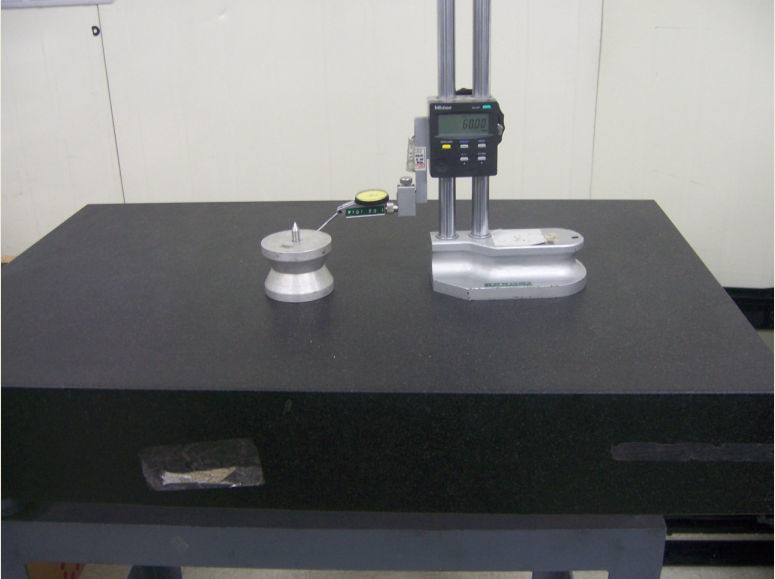
\includegraphics[width=\columnwidth]{Mejagranit}
%                 \caption*{\href{https://commons.wikimedia.org/wiki/File:Mejagranit.jpg}{Blue tooth7}, \href{https://creativecommons.org/licenses/by-sa/3.0}{CC BY-SA 3.0}, via Wikimedia Commons}
%             \end{figure}
%         \end{column}
%     \end{columns}
% \end{frame}

% \begin{frame}
% 	\frametitle{Granite Surface Plates}
%     \begin{columns}
%         \begin{column}{0.48\linewidth}
%             \begin{itemize}[<+- | alert@+>]
%                 \item{Granite is a mix of minerals -- hard quarts, softer mica and feldspar}
%                 \item{Lapping cuts out soft parts, leaves hard projections}
%                 \item{Naturally prevents tools from sticking}
%             \end{itemize}
%         \end{column}
%         \begin{column}{0.48\linewidth}
%             \begin{figure}
%                 \centering
%                 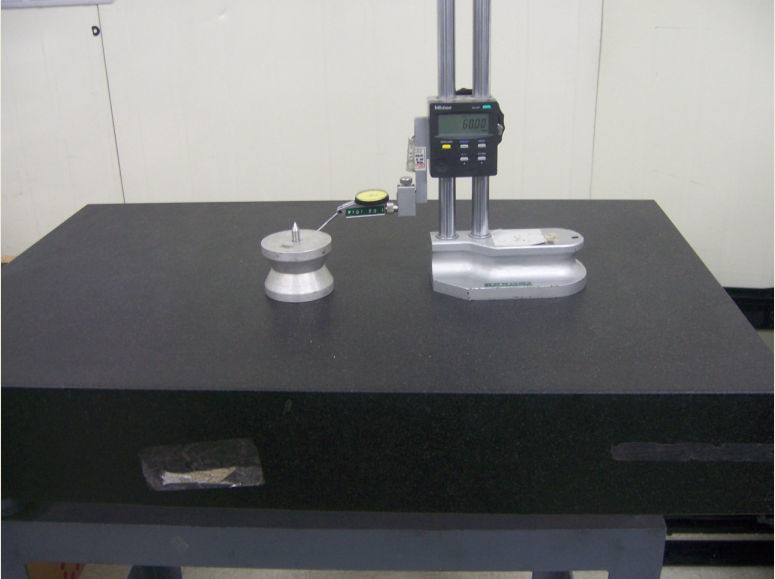
\includegraphics[width=\columnwidth]{Mejagranit}
%                 \caption*{\href{https://commons.wikimedia.org/wiki/File:Mejagranit.jpg}{Blue tooth7}, \href{https://creativecommons.org/licenses/by-sa/3.0}{CC BY-SA 3.0}, via Wikimedia Commons}
%             \end{figure}
%         \end{column}
%     \end{columns}
% \end{frame}

% \begin{frame}
% 	\frametitle{Granite Surface Plates}
%     \begin{columns}
%         \begin{column}{0.48\linewidth}
%             \begin{itemize}[<+- | alert@+>]
%                 \item{Harder than iron}
%                 \item{Shock resistant -- dropping tools won't change shape}
%                 \item{Metal bulges/burrs when scratched -- stone doesn't}
%             \end{itemize}
%         \end{column}
%         \begin{column}{0.48\linewidth}
%             \begin{figure}
%                 \centering
%                 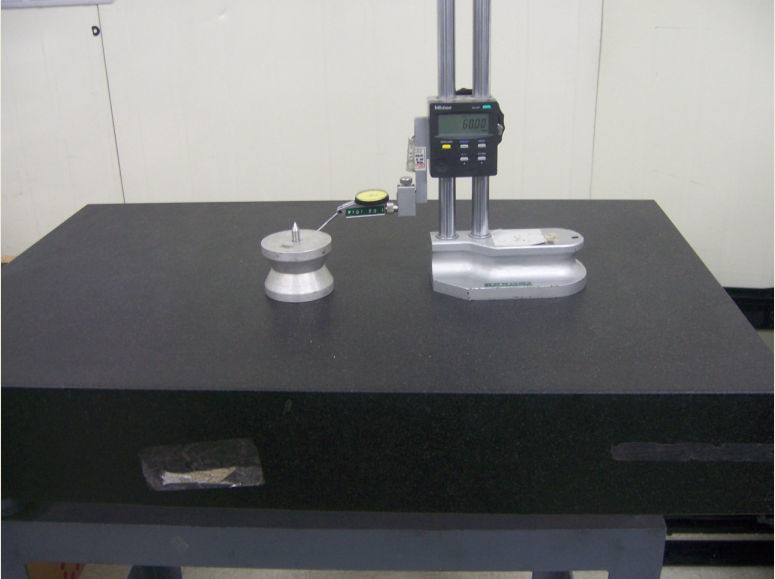
\includegraphics[width=\columnwidth]{Mejagranit}
%                 \caption*{\href{https://commons.wikimedia.org/wiki/File:Mejagranit.jpg}{Blue tooth7}, \href{https://creativecommons.org/licenses/by-sa/3.0}{CC BY-SA 3.0}, via Wikimedia Commons}
%             \end{figure}
%         \end{column}
%     \end{columns}
% \end{frame}

% \begin{frame}
% 	\frametitle{Granite Surface Plates}
%     \begin{columns}
%         \begin{column}{0.48\linewidth}
%             \begin{itemize}[<+- | alert@+>]
%                 \item{Doesn't conduct heat}
%                 \item{Doesn't change size as much as iron with temp changes}
%                 \item{No rust, no corrosion}
%                 \item{Non magnetic}
%             \end{itemize}
%         \end{column}
%         \begin{column}{0.48\linewidth}
%             \begin{figure}
%                 \centering
%                 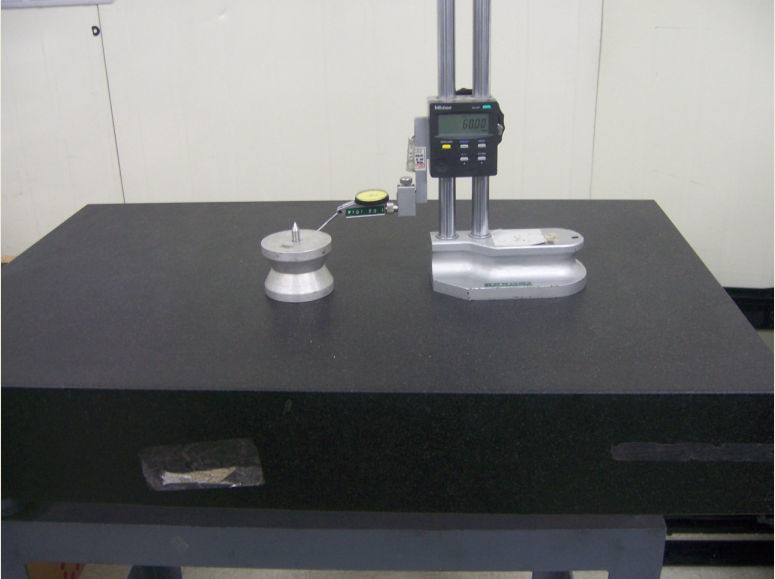
\includegraphics[width=\columnwidth]{Mejagranit}
%                 \caption*{\href{https://commons.wikimedia.org/wiki/File:Mejagranit.jpg}{Blue tooth7}, \href{https://creativecommons.org/licenses/by-sa/3.0}{CC BY-SA 3.0}, via Wikimedia Commons}
%             \end{figure}
%         \end{column}
%     \end{columns}
% \end{frame}

% \section{Surface Plate Accessories}

% \begin{frame}
% 	\frametitle{Surface Plate Accessories}
%     \tableofcontents[currentsection,
%         hideothersubsections
%         ]
% \end{frame}

% \subsection{Parallels}

% \begin{frame}
% 	\frametitle{Parallels}
%     \begin{columns}
%         \begin{column}{0.48\linewidth}
%             \begin{itemize}[<+- | alert@+>]
%                 \item{Rectangular bars of steel ground so that the sides are flat and parallel}
%                     \begin{itemize}
%                         \item{Parallel \textbf{not} square!}
%                     \end{itemize}
%             \end{itemize}
%         \end{column}
%         \begin{column}{0.48\linewidth}
%             \begin{figure}
%                 \centering
%                 \includegraphics[width=\columnwidth]{8642a11p1-a06a-digital@halfx_636880868468773228}
%                 \caption*{\href{https://www.mcmaster.com/}{McMaster-Carr}}
%             \end{figure}
%         \end{column}
%     \end{columns}
% \end{frame}

% \begin{frame}
% 	\frametitle{Parallels}
%     \begin{columns}
%         \begin{column}{0.48\linewidth}
%             \begin{itemize}[<+- | alert@+>]
%                 \item{Can be used to make sure flatness of part being measured}
%                     \begin{itemize}
%                         \item{Top of parallels matches flatness of plate}
%                         \item{If parallels move = no contact = not flat}
%                     \end{itemize}
%             \end{itemize}
%         \end{column}
%         \begin{column}{0.48\linewidth}
%             \begin{figure}
%                 \centering
%                 \includegraphics[width=\columnwidth]{8642a11p1-a06a-digital@halfx_636880868468773228}
%                 \caption*{\href{https://www.mcmaster.com/}{McMaster-Carr}}
%             \end{figure}
%         \end{column}
%     \end{columns}
% \end{frame}

% \begin{frame}
% 	\frametitle{Parallels}
%     \begin{columns}
%         \begin{column}{0.48\linewidth}
%             \begin{itemize}[<+- | alert@+>]
%                 \item{Used when the part being measured would extend below surface plate}
%             \end{itemize}
%         \end{column}
%         \begin{column}{0.48\linewidth}
%             \begin{figure}
%                 \centering
%                 \includegraphics[width=\columnwidth]{8642a11p1-a06a-digital@halfx_636880868468773228}
%                 \caption*{\href{https://www.mcmaster.com/}{McMaster-Carr}}
%             \end{figure}
%         \end{column}
%     \end{columns}
% \end{frame}

% \begin{frame}
% 	\frametitle{Parallels}
%     \begin{columns}
%         \begin{column}{0.48\linewidth}
%             \begin{itemize}[<+- | alert@+>]
%                 \item{Used to protect the surface plate from particularly nasty parts}
%                     \begin{itemize}
%                         \item{Cheaper to replace parallels than surface plate}
%                     \end{itemize}
%             \end{itemize}
%         \end{column}
%         \begin{column}{0.48\linewidth}
%             \begin{figure}
%                 \centering
%                 \includegraphics[width=\columnwidth]{8642a11p1-a06a-digital@halfx_636880868468773228}
%                 \caption*{\href{https://www.mcmaster.com/}{McMaster-Carr}}
%             \end{figure}
%         \end{column}
%     \end{columns}
% \end{frame}

% \begin{frame}
% 	\frametitle{Adjustable Parallels}
%     \begin{columns}
%         \begin{column}{0.48\linewidth}
%             \begin{itemize}[<+- | alert@+>]
%                 \item{Two wedges connected together}
%                 \item{Maintain parallel through range of sizes}
%                 \item{No need for a complete set like above}
%             \end{itemize}
%         \end{column}
%         \begin{column}{0.48\linewidth}
%             \begin{figure}
%                 \centering
%                 \includegraphics[width=\columnwidth]{2211a13p1-a06a-digital@1x_636880859410361516}
%                 \caption*{\href{https://www.mcmaster.com/}{McMaster-Carr}}
%             \end{figure}
%         \end{column}
%     \end{columns}
% \end{frame}            
            
% \subsection{Angle Irons}

% \begin{frame}
% 	\frametitle{Angle Irons}
%     \begin{columns}
%         \begin{column}{0.48\linewidth}
%             \begin{itemize}[<+- | alert@+>]
%                 \item{Originally iron -- modern are steel}
%                     \begin{itemize}
%                         \item{Still called ``angle iron" out of tradition}
%                     \end{itemize}
%                 \item{Surfaces ground flat and at 90$^\circ$ to one another}
%                 \item{Parts can be clamped for measurement at ``perfect" right angle to surface plate}
%             \end{itemize}
%         \end{column}
%         \begin{column}{0.48\linewidth}
%             \begin{figure}
%                 \centering
%                 \includegraphics[width=\columnwidth]{23525a67c1-upA01-1626438971-p9@1x_637620177740046486}
%                 \caption*{\href{https://www.mcmaster.com/}{McMaster-Carr}}
%             \end{figure}
%         \end{column}
%     \end{columns}
% \end{frame}

% \begin{frame}
% 	\frametitle{Angle Irons}
%     \begin{columns}
%         \begin{column}{0.48\linewidth}
%             \begin{itemize}[<+- | alert@+>]
%                 \item{Sides are also ground parallel/square}
%                 \item{Center rib allows it to be clamped down sideways}
%                 \item{Some include bolt holes to mount directly to machines for setup}
%             \end{itemize}
%         \end{column}
%         \begin{column}{0.48\linewidth}
%             \begin{figure}
%                 \centering
%                 \includegraphics[width=\columnwidth]{23525a67c1-upA01-1626438971-p9@1x_637620177740046486}
%                 \caption*{\href{https://www.mcmaster.com/}{McMaster-Carr}}
%             \end{figure}
%         \end{column}
%     \end{columns}
% \end{frame}

% \subsection{V-Blocks}

% \begin{frame}
% 	\frametitle{V-Blocks}
%     \begin{columns}
%         \begin{column}{0.48\linewidth}
%             \begin{itemize}[<+- | alert@+>]
%                 \item{Precision ground on all sides with a V shape on one}
%                 \item{Used to hold round parts}
%             \end{itemize}
%         \end{column}
%         \begin{column}{0.48\linewidth}
%             \begin{figure}
%                 \centering
%                 \includegraphics[width=\columnwidth]{2227a8p1-a01c1585312915-p9@1x_637208917870334506}
%                 \caption*{\href{https://www.mcmaster.com/}{McMaster-Carr}}
%             \end{figure}
%         \end{column}
%     \end{columns}
% \end{frame}

% \begin{frame}
% 	\frametitle{V-Blocks}
%     \begin{columns}
%         \begin{column}{0.48\linewidth}
%             \begin{itemize}[<+- | alert@+>]
%                 \item{Precision ground on all sides with a V shape on one}
%                 \item{Used to hold round parts}
%             \end{itemize}
%         \end{column}
%         \begin{column}{0.48\linewidth}
%             \begin{figure}
%                 \centering
%                 \includegraphics[width=\columnwidth]{2227a8p1-a01c1585312915-p9@1x_637208917870334506}
%                 \caption*{\href{https://www.mcmaster.com/}{McMaster-Carr}}
%             \end{figure}
%         \end{column}
%     \end{columns}
% \end{frame}

% \begin{frame}
% 	\frametitle{V-Blocks}
%     \begin{columns}
%         \begin{column}{0.48\linewidth}
%             \begin{itemize}[<+- | alert@+>]
%                 \item{Many different sizes and styles}
%                 \item{Many include a clamp to hold part in place}
%             \end{itemize}
%         \end{column}
%         \begin{column}{0.48\linewidth}
%             \begin{figure}
%                 \centering
%                 \includegraphics[width=0.9\columnwidth]{382px-V-block_steel}
%                 \caption*{\href{https://commons.wikimedia.org/wiki/File:Surface_plate.jpg}{Rrudzik}, \href{https://creativecommons.org/publicdomain/zero/1.0/deed.en}{CC0}, via Wikimedia Commons}
%             \end{figure}
%         \end{column}
%     \end{columns}
% \end{frame}

% \begin{frame}
% 	\frametitle{V-Blocks}
%     \begin{columns}
%         \begin{column}{0.48\linewidth}
%             \begin{figure}
%                 \centering
%                 \includegraphics[width=\columnwidth]{3117n11p2-a06-digital@1x_636969731756947034}
%                 \caption*{\href{https://www.mcmaster.com/}{McMaster-Carr}}
%             \end{figure}
%         \end{column}
%         \begin{column}{0.48\linewidth}
%             \begin{figure}
%                 \centering
%                 \includegraphics[width=\columnwidth]{3073n11c1-digital1563462350-p9@halfx_636990411728839357}
%                 \caption*{\href{https://www.mcmaster.com/}{McMaster-Carr}}
%             \end{figure}
%         \end{column}
%     \end{columns}
% \end{frame}

% \subsection{Squares}

% \begin{frame}
% 	\frametitle{Squares}
%     \begin{columns}
%         \begin{column}{0.48\linewidth}
%             \begin{itemize}[<+- | alert@+>]
%                 \item{Two pieces, ground to 90$^\circ$ both inside and outside}
%                 \item{\textbf{Beam} -- narrow piece, meant to do the measuring}
%                 \item{\textbf{Base} -- wider piece, meant to go against surface plate}
%             \end{itemize}
%         \end{column}
%         \begin{column}{0.48\linewidth}
%             \begin{figure}
%                 \centering
%                 \includegraphics[width=\columnwidth]{640px-SquareEngineersMachinist}
%                 \caption*{\href{https://commons.wikimedia.org/wiki/File:SquareEngineersMachinist.jpg}{Graibeard}, \href{https://creativecommons.org/licenses/by-sa/2.0}{CC BY-SA 2.0}, via Wikimedia Commons}
%             \end{figure}
%         \end{column}
%     \end{columns}
% \end{frame}

% \begin{frame}
% 	\frametitle{Squares}
%     \begin{columns}
%         \begin{column}{0.48\linewidth}
%             \begin{itemize}[<+- | alert@+>]
%                 \item{Many different sizes available}
%                 \item{Angle irons are meant to fixture parts square, squares are simply meant to measure square}
%             \end{itemize}
%         \end{column}
%         \begin{column}{0.48\linewidth}
%             \begin{figure}
%                 \centering
%                 \includegraphics[width=\columnwidth]{640px-SquareEngineersMachinist}
%                 \caption*{\href{https://commons.wikimedia.org/wiki/File:SquareEngineersMachinist.jpg}{Graibeard}, \href{https://creativecommons.org/licenses/by-sa/2.0}{CC BY-SA 2.0}, via Wikimedia Commons}
%             \end{figure}
%         \end{column}
%     \end{columns}
% \end{frame}

% \begin{frame}
% 	\frametitle{Using a Square}
%     \begin{columns}
%         \begin{column}{0.48\linewidth}
%             \begin{itemize}[<+- | alert@+>]
%                 \item{Look for light}
%                 \item{Use a feeler gauge}
%                 \item{Use a piece of paper}
%             \end{itemize}
%         \end{column}
%         \begin{column}{0.48\linewidth}
%             \begin{figure}
%                 \centering
%                 \includegraphics[width=\columnwidth]{640px-SquareEngineersMachinist}
%                 \caption*{\href{https://commons.wikimedia.org/wiki/File:SquareEngineersMachinist.jpg}{Graibeard}, \href{https://creativecommons.org/licenses/by-sa/2.0}{CC BY-SA 2.0}, via Wikimedia Commons}
%             \end{figure}
%         \end{column}
%     \end{columns}
% \end{frame} 

\begin{frame}
    \frametitle{Image Frame}

    \begin{figure}
        \centering
        \shadowpic[]{0.25\linewidth}{A vintage black and white photograph depicting a woman in profile examining an open manual or book while using a precision mechanical height gauge and dial indicator setup mounted on a surface plate.}{\textbf{Attribution:} Marjory Collins, Public domain, via Library of Congress (\href{https://www.loc.gov/pictures/resource/fsa.8d14582/}{LC-USW3-018540-D})}{service-pnp-fsa-8d14000-8d14500-8d14582v}
    \end{figure}
\end{frame}

\begin{frame}
    \frametitle{Image Frame}

    \begin{figure}
        \centering
        \shadowpic[]{0.25\linewidth}{A vintage black and white photograph showing a woman looking down intently as she operates a precision height gauge with a dial test indicator attached to a metal fixture on a surface plate.}{\textbf{Attribution:} Marjory Collins, Public domain, via Library of Congress (\href{https://www.loc.gov/pictures/resource/fsa.8d14583/}{LC-USW3-018541-D})}{service-pnp-fsa-8d14000-8d14500-8d14583v}
    \end{figure}
\end{frame}

\begin{frame}
    \frametitle{Image Frame}

    \begin{figure}
        \centering
        \shadowpic[]{0.25\linewidth}{A close-up photograph of a metal machine vise holding a small cylindrical metal part using a V-block setup and parallel bars between the vise jaws.}{\textbf{Attribution:} Cdang, \href{https://creativecommons.org/licenses/by-sa/3.0}{CC BY-SA 3.0}, via \href{https://commons.wikimedia.org/wiki/File:Montage_usinage_cylindre_ve_etau.jpg}{Wikimedia Commons}}{Montage_usinage_cylindre_ve_etau}
    \end{figure}
\end{frame}

\begin{frame}
    \frametitle{Image Frame}

    \begin{figure}
        \centering
        \shadowpic[]{0.25\linewidth}{A cast iron V-block standing upright on a blue background, featuring V-shaped grooves on its sides and a blue painted recessed center stamped with the letters R and G.}{\textbf{Attribution:} Romary, \href{https://creativecommons.org/licenses/by-sa/2.5}{CC BY-SA 2.5}, via \href{https://commons.wikimedia.org/wiki/File:Ve_fonte.JPG}{Wikimedia Commons}}{Ve_fonte}
    \end{figure}
\end{frame}

\begin{frame}
    \frametitle{Image Frame}

    \begin{figure}
        \centering
        \shadowpic[]{0.25\linewidth}{A metal V-block clamping a smooth cylindrical metal bar in place with a black top clamp and vertical screw.}{\textbf{Attribution:} Rrudzik, CC0, via \href{https://commons.wikimedia.org/wiki/File:V-block_steel.jpg}{Wikimedia Commons}}{V-block_steel}
    \end{figure}
\end{frame}

\begin{frame}
    \frametitle{Image Frame}

    \begin{figure}
        \centering
        \shadowpic[]{0.25\linewidth}{A pair of metal sine bars of different sizes, each featuring precision cylinders at both ends and weight-reducing relief holes along their bodies, displayed against a light gray background.}{\textbf{Attribution:} Glenn McKechnie, \href{https://creativecommons.org/licenses/by-sa/2.0}{CC BY-SA 2.0}, via \href{https://commons.wikimedia.org/wiki/File:SineBarStyles.jpg}{Wikimedia Commons}}{SineBarStyles}
    \end{figure}
\end{frame}

\begin{frame}
    \frametitle{Tikz Frame}

    \begin{figure}
        \centering
        \resizebox{0.5\linewidth}{!}{
            \begin{circuitikz}[
    american, 
    >={Latex[length=5mm, width=2mm]},
    alt={A diagram illustrating Eratosthenes experimental setup to calculate the circumference of the Earth. A blue circle represents the Earth with a labeled point at the center. Two vertical rods are positioned on the Earth surface, one labeled Rod at Alexandria located at the top and one labeled Rod at Syene located to the upper right. Parallel yellow sunlight rays originate from a yellow circle labeled Sun located at the top right. At Syene, sunlight strikes directly along the vertical line of the rod resulting in no shadow. At Alexandria, the incoming sunlight strikes at an angle relative to the rod, creating a green shadow cast along the curved surface of the Earth. Dashed lines connect the rods to the center of the Earth, forming an central angle theta that matches the angle theta formed between the top of the rod at Alexandria and the incoming sunlight ray.}
    ]

    \fill[
        draw=BakerBlack,
        fill=HitGray,
        fill opacity=0.5,
        ultra thick
    ]
    (0,0)
    -- (0,-2)
    coordinate(A_b_l)
    .. controls (4,-1) and (6,-1) ..
    (8,-2)
    coordinate(A_b_r)
    -- ++(0,2)
    -- (0,0);

    \fill[
        draw=BakerADARed,
        fill=BakerADARed!50,
        fill opacity=0.5,
        ultra thick
    ]
    (A_b_r)
    -- ++(0,-2)
    coordinate(B_b_r)
    -- (B_b_r -| A_b_l)
    coordinate(B_b_l)
    -- (A_b_l)
    .. controls (4,-1) and (6,-1) ..
    (A_b_r);

    \node[
        text=BakerBlack,
        anchor=north west
    ]
    at (0,0)
    {A};

    \node[
        text=BakerBlack,
        anchor=south west
    ]
    at (B_b_l)
    {B};

    \begin{scope}[xshift=9cm]
        \fill[
            draw=BakerBlack,
            fill=HitGray,
            fill opacity=0.5,
            ultra thick
        ]
        (0,0)
        -- (0,-2)
        coordinate(A_b_l)
        .. controls (4,-1) and (6,-1) ..
        (8,-2)
        coordinate(A_b_r)
        -- ++(0,2)
        -- (0,0);

        \fill[
            draw=LakeBlue,
            fill=LakeBlue!50,
            fill opacity=0.5,
            ultra thick
        ]
        (A_b_r)
        -- ++(0,-2)
        coordinate(B_b_r)
        -- (B_b_r -| A_b_l)
        coordinate(B_b_l)
        -- (A_b_l)
        .. controls (4,-1) and (6,-1) ..
        (A_b_r);

        \node[
            text=BakerBlack,
            anchor=north west
        ]
        at (0,0)
        {A};

        \node[
            text=BakerBlack,
            anchor=south west
        ]
        at (B_b_l)
        {C};
    \end{scope}

    \begin{scope}[xshift=4.5cm, yshift=-6.5cm]

        \fill[
            draw=BakerADARed,
            fill=BakerADARed!50,
            fill opacity=0.5,
            ultra thick
        ]
        (0,-0.5)
        -- (0,1.5)
        coordinate(B_t_l)
        -- (8,1.5)
        -- (8,-0.5)
        .. controls (4,-1.5) and (2,-1.5) ..
        (0,-0.5);
        
        \fill[
            draw=LakeBlue,
            fill=LakeBlue!50,
            fill opacity=0.5,
            ultra thick
        ]
        (0,-4)
        -- (0,-2)
        coordinate(C_t_l)
        .. controls (4,-1) and (6,-1) ..
        (8,-2)
        coordinate(C_t_r)
        -- (8,-4)
        coordinate(C_b_r)
        -- (0,-4)
        coordinate(C_b_l);

        \node[
            text=BakerBlack,
            anchor= north west
        ]
        at (B_t_l)
        {B};

        \node[
            text=BakerBlack,
            anchor=south west
        ]
        at (C_b_l)
        {C};

    \end{scope}

\end{circuitikz}
        }
    \end{figure}
\end{frame}

\begin{frame}
    \centering
    {\Huge \textbf{\textcolor{BakerADARed}{Questions?}}}
\end{frame}

\begin{frame}
    \frametitle{Copyright Notice}
    
    {\scriptsize
    \PresTitle \textcopyright 2026 by Brad Peirson is licensed under Creative Commons Attribution-NonCommercial-ShareAlike 4.0 International (CC BY-NC-SA 4.0). To view a copy of the official license, visit \href{https://creativecommons.org/licenses/by-nc-sa/4.0/}{https://creativecommons.org/licenses/by-nc-sa/4.0/}.

    \vspace{0.5em}

    \textbf{Exceptions and Exclusions}

    \begin{itemize}
        \item[Baker College Branding \& Trademarks:]All Baker College logos, trademarks, wordmarks, seals, slide design templates, and proprietary branding elements contained in these materials are \textbf{EXCLUDED} from the CC BY-NC-SA 4.0 license. All rights are reserved by Baker College. Express written permission from Baker College is required for any use, copying, or redistribution of these elements.
        \item[Third-Party Media \& Content:] Any third-party images, graphics, diagrams, or external media incorporated in these materials are included under their respective original licenses or permissions and are individually attributed at their point of use. 
        \item[Original Author Content:] All unattributed figures, diagrams, text, code snippets, and media are original works created by the author and are licensed under the CC BY-NC-SA 4.0 license.
    \end{itemize}

    The appearance of U.S. Department of War (DoW) visual information does not imply or constitute DoW endorsement.
    \par}
\end{frame}

\end{document}

% \begin{frame}
%     \frametitle{Test Todo}

%     % Usage: \tikztodo[width]{height}{description/notes}
%     \tikztodo[0.7\textwidth]{4cm}{Convert block diagram of feedback loop}
% \end{frame}